\documentclass[a4paper]{article} 



% vous pouvez changer les paramètres : voici les options dispoinibles :
% - a4paper
% - fancysections
% - notitlepage ou titlepage
% - onside ou twoside selon si vous voulez l'imprimer en recto-verso ou en recto
% - sectionmark
% - chaptermark (pour les 
% - pagenumber
% - enmanquedinspiration
% en cas de doutes, pas de doutes, la documentation est sur :
%  https://gitlab.binets.fr/typographix/polytechnique/-/blob/master/source/polytechnique.pdf
\usepackage[a4paper,  fancysections,  titlepage]{polytechnique}
\usepackage[english]{babel}
\usepackage[T1]{fontenc}
\usepackage{blindtext}
\usepackage[hidelinks]{hyperref}
\usepackage{amsmath, amssymb}
\usepackage{float}
\usepackage[linesnumbered,ruled,vlined]{algorithm2e}


% nous avons défini deux commandes :
\newcommand{\code}[1]{%
    \mbox{\ttfamily%
        \detokenize{#1}%
    }%
}

\newcommand{\resultat}[1]{%
    \quad \rightsquigarrow \quad #1%
}

\author{Thibaut de Saivre}
\date{\today}
\title{OCM Problem}
\subtitle{Heuristics and solutions}
\logo{typographix}




\begin{document}
\maketitle

\tableofcontents

\begin{figure}[ht]
	\centering
	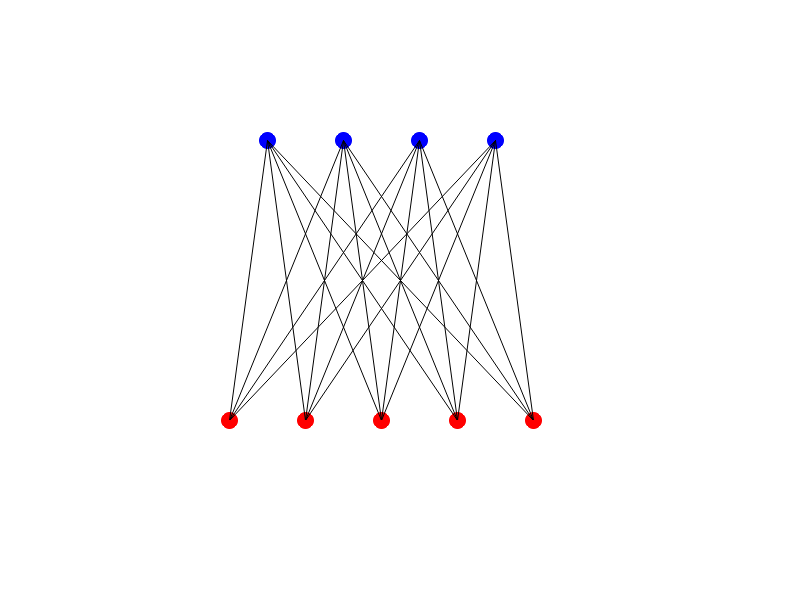
\includegraphics[width=1\textwidth]{images/graph_example.png}
	\caption{An example bipartite graph}
	\label{fig:image1} % Optional label for referencing the figure in text.
\end{figure}

\eject

\section{Algorithms used}

We present here the different algorithms used in this project, with the objective to solve the One Sided Crossing Minimization problem from the \href{https://pacechallenge.org/2024/}{PACE 2024 challenge}. They were implemented in Rust, with GTK windowed display support. See the README.md file for more information.\\

For all graphs, we will consider the following notations:
\begin{itemize}
	\item $V$ the number of vertices
	\item $E$ the number of edges
	\item $C$ the number of crossings
	\item $optimal$ the number of crossings of the optimal solution\\
\end{itemize}

We implemented the following algorithms:\\

\begin{itemize}
	\item Line Sweep crossing counting
	\item Barycentric heuristic
	\item Median heuristic
	\item Iterated Barycentric
	\item Iterated Median
\end{itemize}

\subsection{Barycentric heuristic}

This algorithm as well as the median heuristic one are described in \cite{edgecrossings1994}.

\begin{itemize}
	\item Runtime Complexity: $O(E + V)$
	\item Space Complexity: $O(E + V)$
	\item Solution Optimality: $K \times \text{optimal}$ with $K = \mathcal{O}(\sqrt{V})$
\end{itemize}

For this algorithm, we give every top and bottom node an abscissa depending on their order in their respective horizontal lines in the bipartite graph.
We then update each node's abscissa by taking the average of the abscissas of the nodes it is connected to. If a node has no connections, it keeps its abscissa.

\begin{algorithm}[H]
	\caption{Barycentric algorithm}
	\DontPrintSemicolon
	\KwIn{A bipartite graph}
	\KwOut{A crossing-minimized graph}
	\BlankLine

	\ForAll{nodes}{
		abscissa $\gets$ order in the node's horizontal line\;
	}

	\ForAll{nodes}{
		\eIf{connections > 0}{
			abscissa $\gets$ average of connected nodes' abscissas\;
		}{
			nothing\;
		}
	}

	\ForAll{nodes}{
		abscissa $\gets$ order in the node's horizontal line\;
	}
\end{algorithm}

The algorithm iterates over all nodes and edges not in a nested way, thus it has a runtime complexity of $O(E + V)$.
Note that if you want to associate a rank index to each node of the new graph, you will need to sort the nodes by their abscissa, which has a complexity of $O(V \log V)$.

\subsection{Median heuristic}

Same as the barycentric one, this algorithm is described in \cite{edgecrossings1994}.

\begin{itemize}
	\item Runtime Complexity: $O(E + V)$
	\item Space Complexity: $O(E + V)$
	\item Solution Optimality: $3 \times \text{optimal}$
\end{itemize}

For this algorithm, we give every top and bottom node an abscissa depending on their order in their respective horizontal lines in the bipartite graph,
but instead of updating node abscissas with the average of their neighbors, we take their median. If a node has no connections, it keeps its abscissa. If a node has an even amount of connections, we take the average of the two middle abscissas.\\

\begin{algorithm}[H]
	\caption{Median algorithm}
	\DontPrintSemicolon
	\KwIn{A bipartite graph}
	\KwOut{A crossing-minimized graph}
	\BlankLine

	\ForAll{nodes}{
		abscissa $\gets$ order in the node's horizontal line\;
	}

	\ForAll{nodes}{
		\eIf{connections > 0}{
			abscissa $\gets$ median of connected nodes' abscissas\;
		}{
			nothing\;
		}
	}

	\ForAll{nodes}{
		abscissa $\gets$ order in the node's horizontal line\;
	}
\end{algorithm}

The median of a list of edges can theoretically be computed in $O(n)$ time, but our implementation uses $O(n \log n)$ sorting for simplicity.
However, this detail does not show in the benchmarks.
The algorithm iterates over all nodes and edges not in a nested way, thus it has a runtime complexity of $O(E + V)$.
Note that if you want to associate a rank index to each node of the new graph, you will need to sort the nodes by their abscissa, which has a complexity of $O(V \log V)$.

\subsection{Line Sweep crossing counting}

Before we present the next solving algorithms, we must present the Line Sweep crossing counting algorithm, which is used to count the number of crossings in a graph. It is especially useful for iterative algorithms as a termination criteria, although it is expensive.\\

\begin{itemize}
	\item Runtime Complexity: Worst Case $O((E + V) \times E)$, average case $O((E + V) \log E)$
	\item Space Complexity: $O(E)$\\
\end{itemize}

The idea for this algorithm is to sort edges by order of apparition from to right.
Assuming that top and bottom nodes are numbered starting from 0, this means sorting edges $(i, j)$ in order of $\min(i, j)$.
We then iterate continuously over the node indices, from 0 to $\max(\text{top\_index}, \text{bottom|-index})$, add appearing edges to an \textbf{active edge set} with which we check crossings, and remove disappearing edges from the set.\\


\begin{algorithm}[H]
	\caption{Line Sweep Crossing Counting}
	\DontPrintSemicolon
	\KwIn{A bipartite graph}
	\KwOut{A crossing count}
	\BlankLine

	active\_edges $\gets$ empty set of edges\;
	sorted\_edges $\gets$ sorted edges by $\min(i, j)$\;
	crossings $\gets$ 0\;
	\BlankLine

	\For{index \textbf{in} range(0, max\_index)}{

		Remove disappearing edges from active\_edges (edges with $\max(i, j)$ == current index)\;

		\BlankLine
		\For{each appearing edge \textbf{in} sorted\_edges}{
			crossings $\gets$ crossings + edges in active\_edges crossing the new edge\;
			active\_edges $\gets$ active\_edges + appearing edge\;
		}
	}

	\Return crossings\;
\end{algorithm}

We iterate concurrently over all edges and nodes. In each iteration, we compare the current edge with all currently active edges.
In the worst case, if all edges are active at the same time (very large and transversal crossing pattern), the active edges contain all edges.
The global worst-case complexity thus is $O((E + V) \times E)$. However, in average simple cases, the complexity is closer to $O((E + V) \times \text{average edge span})$, meaning $O((E + V) \log E)$ or even $O(E + V)$.

\subsection{Iterated Barycentric}

The iterated barycentric algorithm consists in repeating the barycentric algorithm multiple times and comparing the crossings count of each iteration to keep the best one.\\
We stop iterating once the number of crossings does not decrease anymore (or even starts increasing). This algorithm is described in \cite{iterative1981}\\

\begin{itemize}
	\item Runtime Complexity: $O((E + V) \times E) \times \text{iterations}$
	\item Space Complexity: $O(E + V)$\\
\end{itemize}

\begin{algorithm}
	\caption{Iterated Barycentric algorithm}
	\DontPrintSemicolon
	\KwIn{A bipartite graph}
	\KwOut{A crossing-minimized graph}
	\BlankLine

	best\_crossings $\gets$ line\_sweep(current\_graph)\;
	new\_crossings $\gets$ best\_crossings\ - 1;
	best\_graph $\gets$ current\_graph\;
	\BlankLine

	\While{new\_crossings < best\_crossings}{
		graph $\gets$ barycentric\_iteration(graph)\;
		new\_crossings $\gets$ line\_sweep(graph)\;
		\BlankLine

		\If{new\_crossings < best\_crossings}{
			best\_crossings $\gets$ new\_crossings\;
			best\_graph $\gets$ graph\;
		}
	}

	\Return best\_graph\;
\end{algorithm}

One advantage of this method is to not give a worse solution than the initial one, because the barycentric method sometimes outputs a worse graph on the first iteration.
The line sweep crossing counting algorithm used after each iteration gives its complexity to this algorithm.

\subsection{Iterated Median}


The iterated median algorithm consists in repeating the median algorithm multiple times and comparing the crossings count of each iteration to keep the best one.\\
We stop iterating once the number of crossings does not decrease anymore (or even starts increasing). This algorithm is described in \cite{iterative1981}\\
It is almost the same as the iterated barycentric algorithm, but with the median algorithm instead of the barycentric one.\\

\begin{itemize}
	\item Runtime Complexity: $O((E + V) \times E) \times \text{iterations}$
	\item Space Complexity: $O(E + V)$\\
\end{itemize}

\begin{algorithm}
	\caption{Iterated Median algorithm}
	\DontPrintSemicolon
	\KwIn{A bipartite graph}
	\KwOut{A crossing-minimized graph}
	\BlankLine

	best\_crossings $\gets$ line\_sweep(current\_graph)\;
	new\_crossings $\gets$ best\_crossings\ - 1;
	best\_graph $\gets$ current\_graph\;
	\BlankLine

	\While{new\_crossings < best\_crossings}{
		graph $\gets$ median\_iteration(graph)\;
		new\_crossings $\gets$ line\_sweep(graph)\;
		\BlankLine

		\If{new\_crossings < best\_crossings}{
			best\_crossings $\gets$ new\_crossings\;
			best\_graph $\gets$ graph\;
		}
	}

	\Return best\_graph\;
\end{algorithm}

This method gives similar results and advantages to the barycentric one.

\eject

\section{Benchmarks}

TODO

\eject

\bibliographystyle{plain}
\bibliography{references}

\end{document}
